
% En esta sección se detallan los experimentos realizados para abordar las cuestiones propuestas en la sección \ref{Introduction}. En primer lugar, se introducen los detalles del diseño de la experimentación: la selección del modelo de segmentación, dataset elegido, procesos de entrenamiento y validación, etc. Después, se detalla el pipeline implementado para realizar la anotación semiautomática de las máscaras de ocupación, oclusión y área conducible. Finalmente, se aborda la metodología seguida para evaluar tanto la generación de las máscaras semánticas en \aclink{BEV}, como las detecciones 3D a partir de imágenes monoculares para la evaluación final del pipeline de anotación semiautomática.

This section details the experiments and implementations made to address the problems described in section \ref{Introduction}. On the first hand, the experimental design is introduced, tackling the model and dataset selection, how data augmentations are performed and the training and validation processes. Afterward, the implementation of the occupancy and occlusion masks preannotation pipeline is presented. Finally, the evaluation strategy of the pipeline is discussed to measure the quality of the resulting semantic masks and the monocular 3D detections for estimating the object's dimensions.

% Este proyecto puede dividirse en 3 bloques principales: experimentación con la segmentación semántica en BEV, diseño e implementación de un sistema de anotación semiautomático de máscaras de área conducible y un tercer bloque de experimentación para evaluar el rendimiento del sistema implementado.

Thus, this project can be divided into three main blocks: \aclink{BEV} semantic segmentation experimentation, design and implementation of the preannotation pipeline and a thrid block of how the system is evaluated.

\subsection{Segmentation experiment design: BEV2Seg\_2}
\label{bev2seg_2}

Para abordar la hipótesis de "Un modelo de segmentación semántica entrenado con imágenes BEV segmenta mejor los elementos planares", se ha diseñado el proceso descrito en la Figura \ref{fig:beg2seg_2_flow}. En él se siguen dos rutas principales: la segmentación de imágenes RGB normales y su reproyección con \aclink{IPM} a BEV y realizar \aclink{IPM} de la imagen original para luego realizar la segmentación semántica con el modelo.

\begin{figure}[h!]
    \centering
    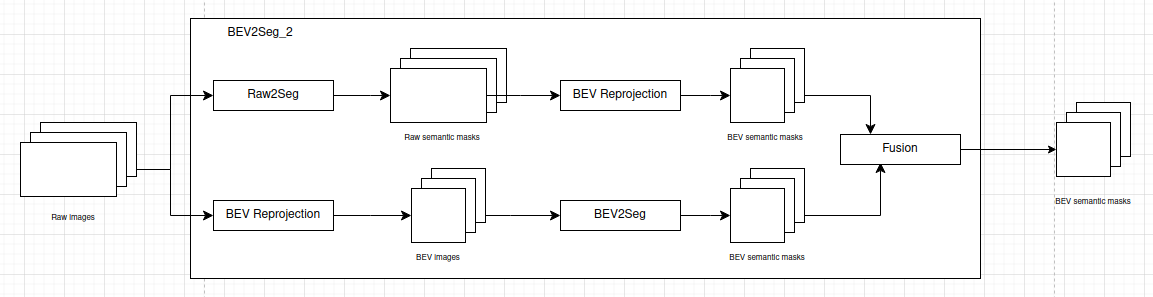
\includegraphics[width=\linewidth]{./images/metodology/bev2seg_2_flow.png}
    \caption{bev2seg\_2 diagram flow}
    \label{fig:beg2seg_2_flow}
\end{figure}

Considerando este diagrama de flujo surgen tres cuestiones principales: (1) qué modelo de segmentación utilizar; (2) con qué base de datos entrenar los modelos y (3) cómo realizar la comparación entre los modelos entrenados.


\subsubsection{Segformer}
Como se ha analizado en el estado del arte \ref{sota}, existen numerosas técnicas para abordar el task de la segmentación semántica y varias de estas técnicas ya se han aplicado al contexto de la segmentación semántica en BEV en el contexto de los \aclink{ADS}. En este punto nos encontramos ante una gran variedad de opciones entre las que elegir. Una de ellas es si optar por modelos CNN o ViT. Tras varias pruebas de distintos modelos \cite{dummy} \cite{dummy} \cite{dummy} se ha tomado la decisión de utilizar segformer \cite{segformer}, un ViT para segmentación semántica que destaca por su eficiencia y rendimiento que consigue resultados del estado del arte.

Explicar cómo funciona segformer por encima.

La estrategia de entrenamiento consiste en utilizar encoders ya entrenados de Segformer y finetunearlos para el task específico: segmentación semántica de escenas vehiculares. Concretamente, encontramos 6 tamaños de encoders MIT (Mix Transformer encoder) de segformer: mit-b0, mit-b1, mit-b2, mit-b3, mit-b4, y mit-b5. Estos encoders están preentrenados en el dataset ImageNet-1K.

La implementación de segformer que se ha seleccionado es la proporcionada por huggingface \cite{huggingface}, ya que cuenta con una API sencilla para entrenar y evaluar los modelos, permite el entrenamiento paralelizado en varias GPU y la utilización de varias CPU y también permite ajustar los hyperparámetros y definir funciones específicas para el entrenamiento.

Para realizar los experimentos, se han utilizado los siguientes encoders y se han añadido los lightweight MLP decoder heads de la siguiente tabla. 

\subsubsection{Dataset}
There are multiple Datasets for the semantic segmentation task on vehicular images such as 
In order to train the model on the segmentation task, a valid dataset must be selected. 

CityScapes [] defines $30$ semantic classes and provides $5000$ frames with pixel-level high-quality annotations and $20000$ weakly annotated images. 

KITTI [] provices $400$ annotated images with a $0.5$ split for training and validation following the CityScape annotation format. 

ApolloScape \cite{ApolloScape} which provides $146.997$ frames with corresponding pixel-level annonations and pose information for 25 labels taken from calibrated cameras whose parameters are available.

NuImages, a subset of NuScenes, contains annotated images on 26 different labels.

There are other benchmarks (cite wildDash and search for others) but in orther to train the models a rich dataset is needed. Despite CityScapes and ApolloScape being good options for this task, NuImages has been selected as it is one of the most used datasets for \aclink{ADS} tasks, it porvided very accurate ego poses and camera parameters and it has a very good documentation.


For all of them, the ego pose and camera parameters metadata are provided. 


\subsubsection{Data augmentations}
\subsubsection{Validación y comparación}
Se ha utilizado mIou per class para la evaluación durante el entrenamiento y la comparación de los dos aproaches.


\subsection{ Driveable area automatic annotation}
\label{aplicacion}

\subsubsection{Depth estimation}
\subsubsection{Scene PCD}
\subsubsection{Instance scene PCD}
\subsubsection{Instance BEV mask}

\subsection{Evaluation methodology}
\label{evaluacion}

\subsubsection{3D detections evaluations}
\subsubsection{BEV masks evaluation}
\hl{se podrían generar las máscaras BEV a partir del groundtruth}


